\chapter{Exploring Fluid Dynamics and the Hagen-Poiseuille (H-P) Equation}
\thispagestyle{fancy}
\fancyhead[RE,LO]{Experiment \thechapter}
%
In this lab we will be analyzing video data gathered previously, using the microscopes, for
fluid flow in two different microfluidic devices.
These microfluidic devices serve as excellent models for fluid flow in biological systems.
By analyzing flow videos in ImageJ, we can explore the effect of device geometry on the velocity, $v$, of the beads in the fluid.
The beads serve as ``tracers'' and tell us how fast the fluid itself is moving.
You will be qualitatively analyzing both devices (see diagram below) and quantitatively analyzing videos from one of these devices.

\begin{figure}[hbtp]
	\centering
	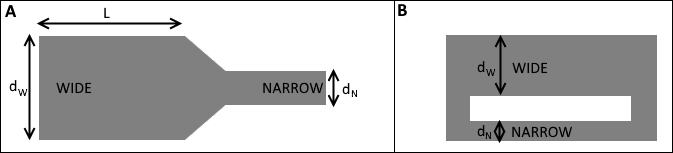
\includegraphics[width=0.8\textwidth]{micro-devices.png}
	\caption{Microfluidic channels in series (A) and in parallel (B).}
	\label{fig:series-parallel}
\end{figure}

Both of the devices consist of two channels connected to each other.
In Device A, the wide and narrow channels are connected in sequence.
In Device B, the wide and narrow channels are next to each other, but both fed from the same inlet and outlet.
In other words, the channels of Device A are in ``Series'' and the channels of Device B are in ``Parallel.''
In these devices, the width, $d$, of the wide channel (6.0 mm) is twice the width of the narrow channel (3.0 mm), and the lengths and depths (not shown in the top view) of the wide and narrow channels on each slide are equivalent.
To drive the fluid through the devices, the video makers used a plunger syringe and applied a force to the plunger that was as steady and repeatable as possible.
\par
As the fluid (containing 5 $\mu$m beads) flows from the left side to the right side of the
microfluidic devices, the volumetric flow rate of the fluid, $Q = v*A$, will be governed by the HagenPoiseuille (H-P) equation:
\[ \Delta P \propto \left( \frac{\mu L}{A^{2}} \right) Q \]
where $L$ is the length of the channel, $\mu$ is the viscosity of the fluid, $A$ is the area of the channel ($A = d*depth$), and $\Delta P$ is the change in pressure between the ends of a channel.

\section*{Part 1: Qualitative Analysis}
To start your investigation (before you begin analyzing videos), look at the motion of the
beads both for the slide of channels in Series (Device A) and for the slide of channels in Parallel (Device B).
These videos are on your computer.
For each device, is the motion faster in the wide channel or in the narrow channel?
For each device, is the pressure drop higher in the narrow or wide channel?
Does this pattern match for the two devices?
Why or why not?
Qualitatively describe what you see and justify/explain why you are seeing what you are seeing using the H-P equation.
Consider what biological systems might be modeled using the Series and Parallel devices.
This portion of the lab may take you 30 minutes or more.
Be thorough!

\section*{Part 2: Quantitative Analysis}
For one of these devices, analyze the videos of the motion of the beads in both the wide and
the narrow channels.
(These videos were collected using a 40X optic and a medium-level resolution (1024 pixels).
The frame rate for each video is in the file name.)
Do a quantitative analysis of these videos (using ImageJ and Excel) to investigate the relationship between the relative widths, d, of the channels and the relative velocities, v, of the beads in those channels.
Is the H-P equation a good description of the relationship?
Why or why not?
What assumptions are we making in our data collection and analysis?
What assumptions are we making in comparing our results to the H-P equation?
Are these assumptions valid?
Do you have enough information to calculate the depth of the channel?
If not, what other information would you need to complete the depth calculation?
Explain your reasoning.
\par
Working together with a lab group that analyzed the other device, make sense of your collective data.
Compare your answers to the questions in the previous paragraph and consider how to answer these questions with respect to the entire data set.
Professional scientists often make use of data collected and analyzed by their peers in order to further their own investigations.
What are some of the factors limiting the adaptation and use of data you have not collected for yourself?